\documentclass{jreport}		% 標準のクラスファイル
\usepackage{paper}			% 神戸高専卒論用のマクロ
\usepackage{graphicx}		% eps等図を取り込むためのマクロ
%\usepackage{times}

\title{電子工学科卒業論文の書き方}	% 卒業論文のタイトル
\author{○○ ○○}			% 報告者
\adviser{○○ ○○}			% 指導教官
\year{○○}					% 年度	

\abstract{
 論文には,表示に続いて論文要旨を記載する。論文要旨は,結果を含めて論文の内容が理解できるように簡潔にまとめられなければならない。論文の構成は,電子工学実験実習で購入した「知的な科学・技術文章の書き方」のP.57に記載されている,分量の少ない場合の論文の場合を参考にすること。また,論文の記載に関しては,本説明を熟読の上,体裁を整えることはもちろんのこと,論文内容も十分に吟味すること。\\
 完成した論文は,A4フラットファイルに下図に示すようにな表示および背表紙を付け,提出すること。
\vspace{1cm}
\begin{center}
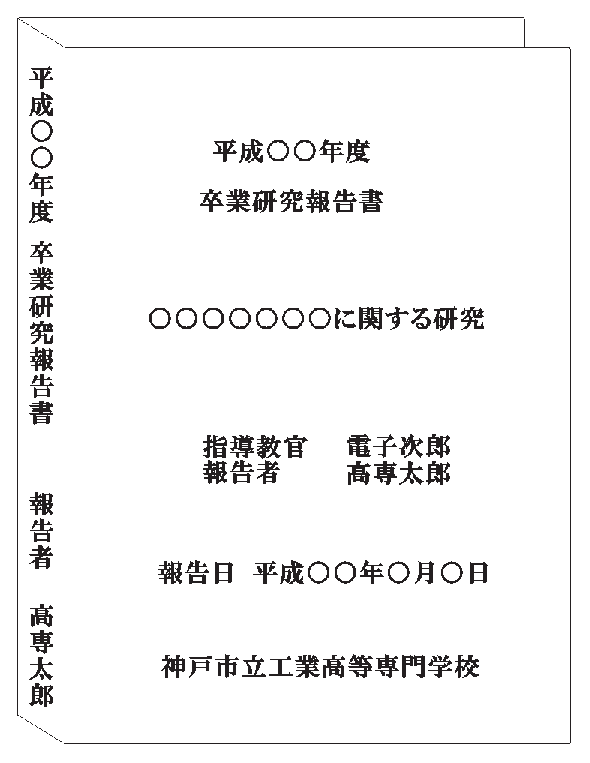
\includegraphics[width=12cm,keepaspectratio,clip]{title.eps}
\end{center}
}%

\begin{document}%
\pagenumbering{roman}
\maketitle		% タイトルページの出力
\tableofcontents	% 目次出力

\chapter{卒業論文の書き方}%
\pagenumbering{arabic}
 ここでは、卒業論文のフォーマットおよび書き方について説明する。卒業論文の基本的な構成や書き方については,前述のように「知的な科学・技術文章の書き方」のP.57に記載されている,分量の少ない場合の論文の場合を参考にすること。なお,論文に掲載する図面や文面は、著作権等を考慮しなければならない。そのため、参考文献の図をコピーしたり、まったく同じ文面を論文に掲載してはならない。論文はオリジナルでなけらばならない。

\section{卒業論文のフォーマット}%
\begin{description}
\item[用紙サイズ] A4縦置きで横書き
\item[枚数] 本文は20ページ以上,30ページ以下とする。資料となるデータ、補足などは本文外の付録とする。(付録は本文分量には含めない)。
\item[余白] 上下右は20mm、左は25mm
\item[書式] 通常文書の使用フォントは10〜11ポイント程度とする。また、
1ページは44文字×40行程度を標準とする。
\item[提出形式] 論文を印刷しA4フラットファイルに綴じて1部提出のこと。また,後日,PDF形式の電子データとして論文を提出してもらう。なお,ファイル名は,「r+学籍番号.PDF」とする。
\item[その他] 論文には,論文要旨(A4, 1ページ),目次を必ず添付すること。
\end{description}

\section{論文の構成}
一般的な卒業論文は,
\begin{description}
\item[表紙] 前述の指定したフォーマットで表紙を作成し,A4フラットファイルに貼り付ける。
\item[論文要旨] 論文内容がわかるように結果を含めて説明する。
\item[目次] 
\item[本文] はじめに(序論),理論,実験方法,実験結果,まとめ(結論)などで構成される。
\item[付録] 実験データ,プログラムなど論文の関係のある資料を添付する。
\item[参考文献] 卒業論文を執筆する上で参考にした資料を記載する。
\item[謝辞] 論文を執筆するにあたり,お世話になった先生や友人にお礼を述べる。
\end{description}
で構成される。詳細については「知的な科学・技術文章の書き方」P.52の卒業論文の書き方を参照のこと。


\section{論文執筆における諸注意}
\subsection{変数および数式の記述方法}
文中には、単位や変数などで英語を用いる場合がある。このとき単位、数学記号にはローマン体、変数には斜体を用いるのが通例である。これは、数式中でも同様である。また,数式には通し番号を付けて整理すること。\par
例1) [A],[cm] \par
例2) $J$ [A], $E$ [eV] \par
例3)
\begin{equation}
f(x) = \log x {\rm [A]}  
\end{equation}

\subsection{図表の書き方}%
図および表の書き方は,「知的な科学・技術文章の書き方」のP.117およびP.163をそれぞれ参考にし,掲載されている悪い例にならないように注意を払うこと。また,図および表には通し番号をつけること。

\subsection{参考文献について}
参考文献の書き方は,「知的な科学・技術文章の書き方」のP.100を参照し,一般的な論文の書き方にしたがって記載すること。

\end{document}
